\section{Reprodutibilidade}

Reprodutibilidade ({\it reproducibility}) é a habilidade de replicar um
experimento ou estudo em sua totalidade a fim de confirmar suas hipóteses, seja
pelo autor original ou por pesquisadores independentes. Esse conceito é um
ponto central do método científico e tem sido uma preocupação crescente da
comunidade de pesquisa em Engenharia de Software Empírica
\cite{gonzalez_reproducibility_2012}.

A verificação de reprodutibilidade é essencial para a prática do método
científico, pesquisadores reportam seus resultados, que são reforçados à medida
que outros grupos independentes da comunidade científica compartilham
resultados semelhantes \cite{mccormick_itk_2014}. Experimentos são repetidos
com objetivo de checar seus resultados, replicações bem sucedidas aumentam a
validade e confiabilidade dos resultados observados no experimento
\cite{almqvist_replication_2006,juristo_replication_2012}.

Apesar do conceito reprodutibilidade ser relativamente concensual entre as
várias áreas da Ciência, existem alguns conceitos similares com uma certa
diferença de significado mas que compõem o debate sobre o tema e são
importantes de serem esclarecidos, segundo
\citeonline{feitelson_repeatability_2015} temos as seguintes definições:

%, diante disto, e preocupado em criar uma linguagem comum entre os
%pesquisadores, \citeonline{feitelson_repeatability_2015} propôs as seguintes
%definições:

\begin{description}

  \item[Repetição ({\it repetition})]
  Refazer exatamente o que outra pessoa fez usando os artefatos originais.

  \item[Replicação ({\it replication})]
  Replicar com precisão exatamente o que outra pessoa fez, recriando os
  artefatos.

  \item[Variação ({\it variation})]
  Repetir ou replicar exatamente o que a outra pessoa fez, mas com alguma
  modificação controlada nos parâmetros.

  \item[Reprodução ({\it reproduction})]
  Recriar o espírito do que outra pessoa fez, usando seus próprios artefatos.

  \item[Corroboração ({\it corroboration})]
  Obter os mesmos resultados de outra pessoa, usando outros meios e
  procedimentos experimentais.

\end{description}

A comunidade de Engenharia de Software tem tentado por anos replicar
experimentos para gerar fragmentos de conhecimento, mas a grande parte
das tentativas tem levado a resultados insatisfatórios (a
credibilidade dos resultados não aumentou), principalmente por conta das
variações nas condições experimentais de uma replicação para outra
\cite{juristo_using_2009}.

Um estudo com 88 papers da conferência {\it MSR (Mining Software Repositories)\footnote{\url{http://msrconf.org}}}
 entre 2004-2011, evidenciou que apenas
62\% são replicáveis ou parcialmente replicáveis e que apenas 20\% dos estudos
disponibilizam suas ferramentas \cite{amann2015software}. Um estudo anterior
com 171 papers do MSR evidenciou que, entre outros problemas, a maioria não
disponibiliza publicamente as ferramentas e {\it scripts}, mesmo quando os autores
explicitamente afirmam que construíram algo \cite{robles2010replicating},
apenas 2 entre 154 estudos experimentais avaliados fornecem os dados e as
ferramentas necessárias para replicação e futuras pesquisas
\cite{barr_shoulders_2010}.

Esta ausência de reprodutibilidade
em estudos científicos baseados em métodos computacionais tem
levado a sérios erros em resultados científicos publicados na literatura acadêmica
\cite{hinsen_activepapers_2015}. O número de repetições apesar de ter crescido nos últimos
anos ainda é muito pequeno, especialmente
considerando a amplitude de tópicos em Engenharia de Software
\cite{silva_replication_2011, kitchenham_evidence-based_2015}.

\citeonline{krishnamurthi_real_2015} em um estudo sobre repetibilidade, chamam
atenção para o papel central que os artefatos de software possuem em pesquisas
da Ciência da Computação e questionam: ``Onde está o software nas pesquisas
sobre linguagem de programação?''.

Em muitos campos científicos onde software tem se tornado ferramenta
fundamental para capturar e analisar dados, este requerimento por
reprodutibilidade implica que plataformas de software e ferramentas confiáveis
e compreensíveis devem estar disponíveis para a comunidade científica
\cite{mccormick_itk_2014}. Toda pesquisa que possua qualquer processo
computadorizado deve publicar seus códigos, eles precisam estar disponíveis,
mesmo que os dados correspondentes não estejam, o código deve estar. De acordo
com o espectro de reprodutibilidade (Figura \ref{reproducibility-spectrum}), a
disponibilidade de código é o requisito mínimo e é o primeiro passo para
possibilitar validação e confirmação dos resultados.

\begin{figure}[h]
  \center
  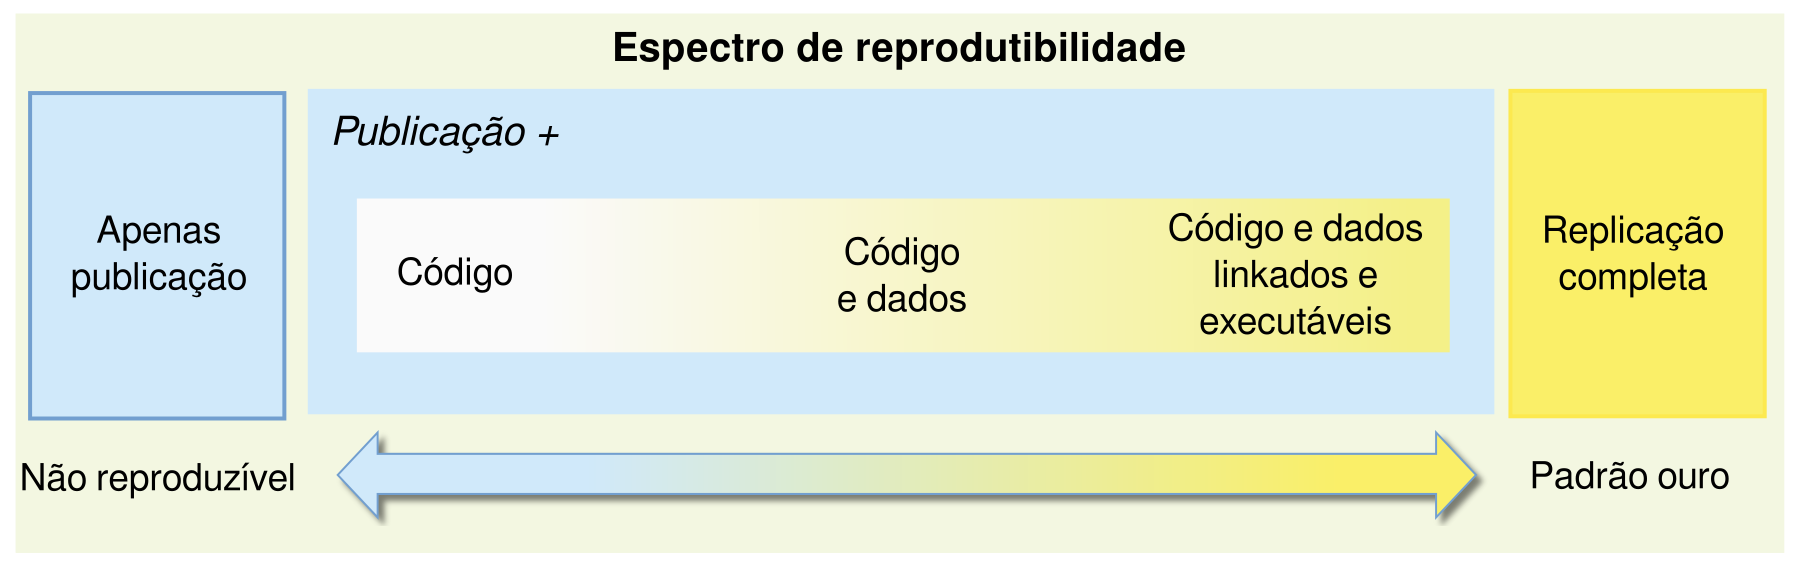
\includegraphics[scale=0.3]{imagens/reproducibility-spectrum-ptbr.png}
  \caption{Espectro de reprodutibilidade \cite{peng2011reproducible}}
  \label{reproducibility-spectrum}
\end{figure}

%\citeonline{vitek_repeatability_2011}
%em um estudo sobre reprodutibilidade e rigor científico destacam a importancia
%de se disponibilizar qualquer material suplementar gerado durante uma pesquisa
%de modo a possibilitar revisores verificarem e replicarem experimentos.

No entanto, esta prática ainda carece de maior adoção, as questões por trás
destes problemas são, além de outros, possivelmente, ocasionados por questões
culturais \cite{niemeyer2017open}, como, por exemplo, a tímida adoção de
práticas da ciência aberta entre pesquisadores.

\subsection{Ciência Aberta}

Ciência Aberta é um movimento que tem por objetivo tornar a pesquisa
científica, seus dados e sua disseminação acessíveis à todos os interessados,
sejam amadores ou profissionais \cite{WikipediaOpenScience}. Sua principal
motivação está em possibilitar a reprodução dos resultados de pesquisas e em
garantir transparência das metodologias utilizadas, isto aumenta o impacto
social das pesquisas e gera economia de tempo e dinheiro para os pesquisadores
e para as instituições \cite{nesta2010open}.

Este movimento é guiado por princípios básicos de transparência, acessibilidade
e reusabilidade universais, disseminadas via ferramentas online, ele é dividido
em quatro grandes áreas: (1) {\it Open Access}, (2) {\it Open Data}, (3) {\it
Open Source} e (4) {\it Open Reproducible Research}.

%Dentre elas destaca-se a Open Reproducible Research
%por preocupar-se com a reprodutibilidade dos resultados de pesquisas de forma
%independente \cite{stodden2009} e aberta, no entanto, esta área tem recebido
%ainda pouca atenção da comunidade de pesquisa \cite{Nancy2015}
%\cite{Grand2010Open} apesar do aumento geral do interesse pelas práticas da
%Ciência Aberta \cite{Grand2010}.

A Ciência Aberta pode ter praticado tanto por razões filosóficas quanto
pragmáticas. Como os recursos produzidos por projetos abertos são
potencialmente acessíveis ao público público, a Open Science oferece um meio
inovador para acesso público e envolvimento no processo de Ciência e um método
inovador para comunicação científica em tempo real. Esse acesso direto limpa o
fluxo de comunicação ou enlameia as águas com comentários não focados, pouco
claros e sem conta? Este artigo sugere que a adoção de uma abordagem Open
Science permite a captura de um registro de pesquisa autêntico e claro. No
entanto, os pesquisadores reconhecem que isso envolve a abertura de seu
trabalho a um tipo diferente de escrutínio
\cite{grand_open_2010}.

A Open Science é uma abordagem emergente para a condução de projetos de
ciência, tecnologia e engenharia, em que informações sobre toda a pesquisa em
andamento estão disponíveis e através da Internet. Adotar uma Abordagem de
Ciência Aberta significa que a audiência para a pesquisa pode se estender além
dos estudiosos envolvidos para outros pesquisadores e para os membros do
público. Assim, a Open Science tem implicações para pesquisa de engenharia,
prática, publicação e engajamento público com engenharia. Este artigo analisa a
história e a evolução do movimento da Ciência Aberta, inclui algumas reflexões
sobre as áreas relacionadas de Acesso aberto, revisão por pares e envolvimento
público com ciência e engenharia e discute dados coletados de entrevistas. A
análise sugere que você tenha preocupações sobre questões como precedência e
proteção do trabalho original e o tempo necessário para integrar práticas
científicas abertas no trabalho diário. Trabalhar com êxito em tais
colaborações provavelmente exigirá não apenas ferramentas práticas comuns, mas
também o desenvolvimento de linguagem compartilhada e compreensão entre
pesquisadores e membros do público. Os entrevistados reconhecem o valor da Open
Science em pesquisas colaborativas e suas facilidades inovadoras para sustentar
o acesso público direto aos resultados da pesquisa. Também tem o potencial de
permitir que os membros do público façam verdadeiras contribuições práticas
para a pesquisa \cite{grand_open_2010}.

%%%%%%%%%%%%%%%%%%%%%%%%%%%%%%%%%%%%%%%%%%%%%%%%%%%%%%%%%

%Over the past fifteen years the scholarly communications agenda
%has progressed gradually. Currently we are experiencing a strong
%tendency among all research stakeholders to engage with the
%practice of OS. Lately, research funders require the sharing not
%only of the research results they have funded, but also of the
%procedures and data that are being generated during the research
%conduct. Researchers, on the other side, are keen on observing
%their research results being used for the improvement of the
%society and are forced by their funders to demonstrate the impact
%of their research. At the same time, higher academic institutions
%aim to join the OS agenda as well, since they see the opportunity
%of great economic benefits and savings. While OS is the possible
%answer to all these factors, the stakeholders’ inability to
%understand the requirements for the application of OS can be a
%suspensory factor for the OS implementation and evolution.
%The aim of the FOSTER project is to advance the stakeholders'
%knowledge on the usefulness of OS and explain the technicalities,
%strategies and best practices using which OS can be applied. As an
%attempt to educate the largest number of researchers possible,
%FOSTER has created an e-leanring portal, which contains quality
%assured information relating to the topic and it is open to everyone
%in the world. The platform contains two types of information:
%learning material and online courses. The classification of these
%two types is supported by an OS taxonomy, where related terms
%are applied both in the portal's material and also in the courses.
%With the use of the taxonomy, users are in the position to
%understand the OS domain and the concepts around it.
%The main goal of the FOSTER project, which is mainly achieved
%through the portal functionalities, is not only to educate the
%research stakeholders on OS, but also to build a community of
%researchers, librarians, software developers, funders and research
%administrators who are interested in OS in order to advance the
%way research is being conducted and shared. In addition, FOSTER
%attempts to provide tools to this community, such as re-usable
%content for training and a platform for blended learning and e-
%learning courses that the community could run. This OS
%advancement is essential for the research promotion and,
%consequently, for the benefit of the society as a whole
%\cite{Nancy2015}.


%\subsection{Software como cidadão de primeira classe}

%Diversas maneiras de inventivar citação formal entre artefatos digitais,
%software por exemplo, tem surgido, dentre elas uma iniciativa interessante
%é o Journal of Open Source Software (JOSS) é um livre a open-access jornal para
%publicação de artigos descrevendo software acadêmico. Ele tem dois objetivos
%principais, melhorar a qualidade dos softwares submetidos e prover mecanismos
%para pesquisadores desenvolvedores de software acadêmico receber crédito pelos
%seus softwares. Enquanto pensado para trabalhar dentro do atual sistema de
%mérito da ciência, JOSS visa a escassez de recompensas para contribuições
%importantes para a ciência realizadas em forma de software. JOSS publica
%artigos que encapsulam sabedoria contida no software ele mesmo, e seu rigoroso
%revisão em pares mirado nos componentes do software: funcionalidade,
%documentação, testes, integração contínua, e a licença. Um artigo JOSS contém
%um resumo descrevendo o objetivo e funcionalidades do software, referencias, e
%um link para o software archive.  O artigo é um ponto de entrada para
%submissçao que engloba o conjunto completo de artefatos de software. Artigos
%aceitos no JOSS recebem um digital object identifier (DOI), te seus metadados
%depositados no Crossref, e o artigo pode começar a colecionar citações e ser
%indexados em serviços como Google Scholar e outros. No seu primeiro ano,
%iniciado em Maio de 2016, JOSS publicou 111 artigos, com mais de 40 artigos
%adicionais sob revisão \cite{smith2017journal}.

%FORCE11 Software Citation principles \cite{smith2016software}\footnote{\url{https://www.force11.org/software-citation-principles}}
%Enfatiza persistencia e claridade e diz que ``Software deve ser considerado
%um produto legítimo de pesquisas e devem ser possível de serem citados''.

% Software Carpentry: lessons learned [version 2; referees: 3 approved]
%
% iniciativa voltada a melhorar as habilidades com computação entre os
% pesquisadores de diversas áreas, ajudando a melhorar os resultados,
% facilitar reprodutiblidade, acesso a dados, codigos, etc... reducao de custos
% melhoria de qualidade, etc... faz workshops, eventos, treinamentos, ao longo
% dos varios anos de existencia, ...
%
% Since its start in 1998, Software Carpentry has evolved from a week-long
% training course at the US national laboratories into a worldwide volunteer effort
% to improve researchers' computing skills. This paper explains what we have
% learned along the way, the challenges we now face, and our plans for the
% future.

% (6) A systematic literature review of software product line management tools \cite{pereira2015systematic}
%
% (???)
%
% (7) Software configuration management tools \cite{chan1997software}
%
% (???)

%A situação com software é amplamente análoga (mas não identica) ao de dados
%das publicações; de fato, todo dado é processado por softwares de alguma forma
%(Borgman et al., 2012).

%\item The GeoScience paper of the future initiative \cite{OntoSoft2016}\footnote{\url{http://www.scientificpaperofthefuture.org/gpf/what-is-a-gpf}}
%Possui um conjunto de requerimentos para softwares serem incluidos em
%papers.  Focando mais no paper em sí do que no software.

%\item UK RSE \cite{ukrse2013}\footnote{\url{http://rse.ac.uk/who}}
%Conscientização sobre a importância e o papel do {\it Research Software
%Engineer} através de comunicação e suporta institucional.

%Science rests on peer review and the wide-spread dissemination of
%knowledge. Software engineering research will advance further and
%faster if the sharing of data and tools were easier and more wide-
%spread. Pragmatic concerns hinder the realization of this ideal: the
%time and effort required and the risk of being scooped. We examine
%the costs and benefits of facilitating sharing in our field in an effort
%to help the community understand what problems exist and find
%a solution. We examine how other fields, such as medicine and
%physics, handle sharing, describe the value of sharing for replication
%and innovation, and address practical concerns such as standards
%and warehousing. To launch what we hope will become an ongoing
%discussion of solutions in our community, we present some ways
%forward that mitigate the risk of sharing — partial sharing, registry,
%escrow, and market \cite{barr2010shoulders}.

%A ciência aberta e comunidades de pesquisa em software tem sido bastante ativas
%em criar manifestos visando chamadas para ação. Estes manifestos chamam para melhorar
%os softwares e os metadados de bibliografia para citação persistente destes softwares.
%Outros tópicos endereçados nestes manifestos incluem ênfase no acesso ao código fonte.

%Isto contradiz as boas práticas de qualquer projeto experimental ({\it
%laboratory
%notebooks}\footnote{\url{https://en.wikipedia.org/wiki/Lab_notebook}}, dados
%organizados, passos documentados, projeto estruturado para reprodutibilidade) e
%torna praticamente impossível utilizar o método mais comum e cientificamente
%produtivo de produzir conhecimento novo a partir de pesquisas anteriores, a
%replicação, ou seja, seguir os mesmos passos do autor original com
%objetivo de validar, melhorar ou estender seus dados e sua metodologia
%\cite{king1995replication, Stodden2010}.

%Análise de imagens médicas é um campo
%em que o uso do recurso computacional, tanto software quanto hardware, são plataformas essenciais
%para realizar trabalho experimental. Nesta arena, a introdução do 
%Insight Toolkit (ITK) em 1999 transformou o campo e facilitou o seu progresso acelerando
%a taxa em que implementação de algoritmos são desenvolvidos, testados e disseminados e
%melhorados. Sendo construído com a eficiência e qualidade das metodologias de
%siftware aberto, ITK
%tem proporcionado a comunidade de imagem médica com uma plataforma efetiva onde constroi
%um workflow diário que incorpora as verdadeiras práticas científicas de reproducibility verification.
%Este artigo descreve os mútiplas ferramentas, metodologias, e prpaticas que a comunidade ITK
%adotou, refinou, e seguiu durante a última década, chegando a se tornar uma das comunidades
%de pesquisa com a maior e moderna infraestrutura de verificação de reprodutibilidade. Por exemplo,
%207 contribuidores criaram 2400 testes unitários que proporciona mais de 84\% de cobertura de teste de linhas.
%O Insight Journal, um periódico de publicação aberta associado com o conjunto de ferramentas (toolkit),
%tem visto mais de 360.000 downloads de publicações. A média normalizada próximo a centralidade, a medida de fluxo
%de conhecimento, resultando de uma distruído revisão em pares de código do sistema foi maior 0.46
%\cite{mccormick_itk_2014}.

%Este artigo reporta
%a primeiras conclusões do projeto ActivePapers, que possui objetivo de desenvolver e aplicar
%uma plataforma computacional que permite publicação de pesquisa computacional em forma que
%habilite instalação-free deployment, encorajando reuso, e permitindo integração completa de dataset e software
%nos registros científicos. O principal conclusão é que estes objetivos podem ser
%atingidos com tecnologia existente, mas que não existe caminho direito para adaptar software legado para este
%framework
%\cite{hinsen_activepapers_2015}.

%Um fator em favor da aceitação dos conceitos da EBSE tem sido a crescente
%reconhecimento que os resultados de estudos empíricos individuais são frequentemente
%inconclusivos, e estes tipo de estudos são difícels de replicar com sucesso
%\cite{sjoberg2005survey}.

%O método científico moderno baseia-se no uso da refubabilidade como critério
%para demarcar o que é Ciência empírica daquilo que não é Ciência empírica.
%Empirismo na filosofia da Ciência enfatiza a evidência, especialmente porque as
%descobertas são resultado de experiências. É uma parte fundamental do método
%científico que todas as hipóteses e teorias devem ser testadas contra
%observações do mundo natural, em vez de descansar apenas em um raciocínio a
%priori, a intuição ou revelação.

%Entre 20 replicações, cinco podem ser consideradas close replications na
%terminologia de Lindsay e Ehrenberg [31], ou seja,
%uma tentativa to retain, tanto quanto é possível, grande parte do conhecimento
%condições do original experimento.
%\cite{sjoeberg_survey_2005}

%Entre estudos de engenharia de software empírica, os que são baseados em dados
%coletados de repositórios de desenvlvimento (como gerenciamento de código-fonte, issue tracking ou
%sistemas de comunicação) são especialmente adequados para reprodução.
%Entretanto os seus status de reprodutibilidade pode variar bastante, de fácil para
%quase impossível de reproduzir. Este artigo explora quais elementos podem ser considerados para
%caracterizar a reprodutibilidade de um estudo nesta área, e como eles podem ser analisados
%paraa melhor entender o tipo de estudos de reprodução eles podem habilitar ou obstruir.
%Um dos principais resultados desta exploraçao é a necessidade de uma abordagem sistemática
%para avaliar a reprodutibilidade de um estudo, dado a complexidade dos processos usualmente envolvidos,
%e da grande quantidade de detalhesq ue devem ser levadas em consideração. Para atingir esta necessiadde,
%uma metodologia para avaliar a reprodutibilidade de estudos também foi apresentada e discutida,
%como uma ferramenta para 
%ajuda a aumentar a conscientização sobre a reprodutibilidade da pesquisa neste campo.
%A aplicação da metodologia em prática mostrou como, mesmo para artigos apontados como reproduzíveis,
%uma análise sistemática mostrou importante aspectos que fazem reprodução difícil ou impossível.
%Nós também mostramos como, identificando elementos e atributos relacionados a reprodutibilidade,
%isto pode ser melhor entendido com um tipo de reprodução pode ser feita para um estudo específico, dado
%a descrição dos dadasets, metodologia e  parametros que foram usados \cite{gonzalez_reproducibility_2012}.

%Reproducibility manifesto \cite{Barba2012}\footnote{\url{http://lorenabarba.com/gallery/reproducibility-pi-manifesto}}
%Inclui termos para fazer softwares reusáveis por outros. Foco em
%reprodutibilidade, deixando sustentabilidade de software fora de questão.

%Afirmo que o que muitos no campo estão advogando é a replicability dos
%experimentos publicados. Eles argumentam que isto atinge os requisitos de reproducibility
%inerentes da ciência. Minha reclamação é que replicability é um primo pobre substitituto para
%a reproducibility científica. Devem existir outras boas razões para
%a coleção de software e scripts que são as bases de resutados experimentais
%publicados em artigos mas a reproducibility científica não é uma delas
%\cite{drummond_replicability_2009}.

%... Ten Simple Rules for Reproducible Computational Research
%... \cite{sandve_ten_2013} ...

%Variações nao desejadas nas condições do experimento são consequencia
%da extrema dificuldade em descrever um experimento em SE em detalhes suficientes para ouotro
%pesquisador controlar a configuração (setting) e replicar it exatamente. QUando
%o contexto do experimento é facilmente controlado (o que é muito fácil para o mesmo pesquisador
%no mesmo ambiente e settings), replicações tem satisfatoriamente sucesso.
%Isto é muito rato de controlar apropriadamente a replicação contexto em campos imaturos com experimentação
%lidando com humanos trabalhando em complex settngs., como SE. O contexto do experimento na SE cobre hundreds de variáveis
%e nós não sabemos ainda quais tem maior importancia.
%
%Por conta do contexto tão complexo, muita informaçao é necessária sobre o experimento se
%isto for satisfatoriamente replicado. Por exemplo, quando replicando experimentos sobre técnisas de 
%design em SEm não apenas os presuisadores precisam conhecer quais técnicas são examinadas
%mas também como as técnicas são aplicadas, como os sujeutos são treinados, quais conhecmentis
%estes sujeitos já possuem, etc.
%Para jaudar experimentadores a repetir SE experimentos com exatidao quanto possível,
%pacotes de replicação tem sido desenvolvidos. Eles transmitem as informações necessárias sobre o
%experimento pra outros experimentadores. A informação que o pacote de replicação devem conter
%evoluiu ao longo dos anos as shown in [3], [9], [15], [16].
%\cite{juristo_using_2009}

%Existe um debate sobre o melhor caminho para rodar replicações em experimentos de Engenharia de Software.
%Algumas das questões que tem cropped up neste debate são, "Os replicadores devem reusar
%o baseline experiments materials? Qual é a forma de comunicação adequada entre
%experimentalistas e replicadores, se é que há algum? Quais elementos da estrutura experimental
%podem ser alteradas e ainda serem consideradas replicação ao invés de um novo experimento?"
%\cite{juristo_replication_2012}.
%Um entendimento profundo sobre os conceitos de replicação deve ajudar a clarificar essas questões tão bem quanto
%aumentam e melhoram replicações em práticas de Engenharia de Software experimental.
%\cite{juristo_replication_2012}

%Replicaçao de experimento é uma feature chave da experimentação em todo
%campo científico e tecnológico. Intuitivamente, replicação significa repetição de um experimento
%para checar os seus resultaos.
%\cite{juristo_using_2009}.


%Mesmo com estes pacotes
%entretando, muitos estudos tem chamado atenção para o fato que ainda poucos repicação em SE.
%Por alguma razao, pacotes experimental não são tão úteis quanto se esparava ser.
%Também, há autores contra o uso de pacotes experimentais. Isto sugere que nós devemos lidar com este priblema
%em SE experimentos replication from naive perspective.
%\cite{juristo_using_2009}
%
%Entretanto, Kitchenham alerta sobre o mesmo problema que podem atingit replicação e compartilhamento \cite{kitchenham_role_2008},
%em particular quando reuso aos chamados laboratory packages.
%Se estes pacotes são apenas coletados uma vez e reusado muitas vezes,
%isto pode amplificar prováveis erros que ocorrem durante a fase de coleta. A
%disponibilidade de conjunto de dados (dataset) não removem a necessidae de novos datasets,
%que podem ser usados para testar a corretude (correctness) de resultados anteriores.
%Em muitos casos, isto não invalida o argumento anterior: estudos sobre evolução de software
%devem ser replicáveis, seja reusando datasets e ferramentas (tools) de terceitos, seja
%fazendo seus dados ou tools publicamente disponíveis.
%\cite{herraiz_evolution_2013}

%Apesar das pesquisas reproduzíveis ({\it RR - Reproducible Research}) não
%resolverem todos os problemas de validade experimental dos estudos em
%engenharia de software, elas ao menos garantem que dados e métodos de análise
%estejam disponíveis para inspeção e que os resultados possam ser derivados,
%facilitando revisão logo que a publicação acontece.
%\cite{madeyski_would_2017}.

%softwares acadêmicos são, muitas vezes, mal
%documentados, não intuitivos e difíceis de instalar, uma fração substancial são
%abandonware, ou seja, não são mais mantidos ou desenvolvidos ativamente, mesmo
%tendo um valor potencial para a comunidade científica \cite{list_ten_2017}

%Em
%2012, um workshop intitulado ``{\it Reproducible Research: Tools and Strategies for
%Scientific Computing}'' \cite{stodden_reproducible_2012} discutiu, especificamente, iniciativas
%e ferramentas voltadas a apoiar pesquisas reprodutíveis.

%\citeonline{stodden_researchcompendia_2015} demonstram o
%projeto "ResearchCompendia.org", uma infraestrtura para reprodutibilidade e
%colaboração em ciência computacional.

%Apenas quando o mesmo pesquisador realizar a replicação no mesmo local "site" o sucesso
%da replocaão é atingido \cite{juristo_using_2009}.

%Além destes e tantos outros estudos em
%\cite{github2016reproducibility} é possível acessar um guia sobre como
%desenvolver pesquisas cientíticas de forma que promovam a reprodutibilidade.

%Em várias conferências de machine learning, em vários momentos, existem discussões
%a respeito da inabilidade de replicar resultados experimentasis publicados em artigos.
%Parece haver uma visão ampla que nós precisamos de algo para lidar com este problema,
%visto como algo essencial para o avanço do nosso campo. 
%O argumento mais convincente parece ser que a reprodutibilidade dos resultados experimentais é a marca registrada da ciência.
%Entretando, dado que a maioria de nós respeita machile learning como uma disciplina
%científica, ser capaz de replicar experimentos é primordial.
%I quero desafiar esta visão separando a noção de 
%reproducibility, uma propriedade geralmente desejada, de 
%replicability, seu primo pobre. Afirmo que exuste diferenças importantes
%entre os doois.  Reproducibility requer mudanças, 
%replicability evita elas. Entretando reproducibility é desejado, afirmo que
%uma versão melgorada, replicability, não vale a pena ter
%\cite{drummond_replicability_2009}.

%A ciência caminha sob a teoria e experimentação. Não existe ciência fechada \cite{vardi_science_2010}.

%A replicação de um experimento
%produz novos resultados, que, através de comparação com os resultados do
%experimento original (ou outras replicações), aumentam ou decrementam a
%credibilidade dos resultados \cite{juristo_using_2009}.

%. Após várias replicaçãoes
%tendo aumentado a credibilidade de resultados, o pequeno fragmento de
%conhecumento que o experimento está tentando validar é mais maduro. Este
%caminho, replicação ajuda a produzir um corpo experimental de conhecimento
%\cite{juristo_using_2009}.

%Incentivo para realizar replicações externas
%e padrões melhores para relatar estudos empíricos e suas repetições ainda são
%necessárias \cite{silva_replication_2011}.

%, alguns publicados
%recentemente "2014". Muitas estratégias são atualmente perseguidas para
%melhorar a situação \cite{hinsen_activepapers_2015}.

%Apesar da preocupação com a reprodutibilidade dos resultados de pesquisas de
%forma independente \cite{stodden2009enabling} e aberta, esta área tem recebido ainda
%pouca atenção da comunidade de pesquisa \cite{pontika_fostering_2015,grand_open_2010}.

%Uma teoria da evolução de software
%deve se basear em resultaados empíricos, verificáveis e reproduzíveis, e feito
%em larga escala, só assim conclusões com significância estatística podem ser alcançadas.
%Se evolução de software é analisada com dados que não estão disponíveis para terceiros,
%ele não pode ser verificado, repetido ou replicado. É perigoso construir uma teoria
%em cima de estudos empíricos que não cumprem estes requerimentos.
%Estudos empíricos sobre evolução de software devem estar em conformidade com
%guidelines sugeridos para engenharia de software empírica
%\cite{kitchenham_preliminary_2002, kitchenham_role_2008}.

%Estes são alguns problemas relacionados aos softwares acadêmicos, muitos são
%resultado de baixos orçamentos, limitação de tempo e alta rotatividade entre os
%grupos de pesquisa, outros são,

%Compreender os reais motivos
%por trás destes problemas seria, naturalmente, o passo essencial para solucioná-los,
%apesar disso, antes mesmo de resolver tais questões é
%fundamental compreender os impactos que eles causam na comunidade de pesquisa.

%Mesmo sabendo que todo artefato tem impacto na reprodutibilidade
%\cite{gonzalez_reproducibility_2012}, uma barreira comum para tal prática, e
%consequentemente para repetição, replicação e variação é a indisponibilidade do
%código fonte.

%\citeonline{stodden2009enabling} preocupada com as barreiras legais para
%disponibilidade de artefatos de pesquisa propõe o framework ``{\it Reproducible
%Research Standard (RRS)}'', onde sugere formas de usar o licenciamento e as leis
%de copyright da melhor forma para manter disponíveis os produtos gerados
%durante pesquisas e assim viabilizar reprodutibilidade.

%Além disso, é um recurso valoroso para pesquisadores iniciantes, pesquisas
%reproduzíveis melhoram o impacto do próprio estudo, por exemplo, artigos de
%computação que não disponibilizam pubicamente dados e códigos possuem menos
%chances de serem citados \cite{madeyski_would_2017}.

%Diante disso \citeonline{peng2011reproducible} sugere adotar soluções
%intermediárias, repetição, replicação, variação, e desta forma já teríamos uma
%grande melhoria sobre a 

%, estas ferramentas irão empoderar eles e o público para
%verificar, através da prática, a reprodutibilidade das observações que foram
%reportadas na literatura científica \cite{mccormick_itk_2014}.

%Áreas de estudo como a de aprendizado por máquina e
%evolução de software tem levantado preocupações neste sentido
%\cite{kitchenham_preliminary_2002, kitchenham_role_2008,
%drummond_replicability_2009}.

%, aumentando também o
%impacto social das pesquisas, gerando economia de tempo e dinheiro para os
%pesquisadores e para as instituições \cite{nesta2010open}.

%A situação atual onde muitos estudos em engenharia de
%software sofrem de dificuldades de repetição \cite{tang2016worthiness} e,
%consequentemente, poucos estudos replicando pesquisas da área são encontrados.


%% Enquanto pesquisadores publicam artigos descrevendo e divulgando seus
%% resultados, é raro que façam o mesmo com toda a produção gerada durante a
%% pesquisa. A maioria dos componentes necessários para a reprodução dos
%% resultados de uma pesquisa -- por exemplo, códigos fonte e dados -- usualmente
%% permanecem não publicados. Esse problema fere um dos fundamentos
%% da ciência de que novas descobertas sejam reproduzidas antes de serem
%% consideradas parte da base de conhecimento \cite{stodden2009enabling}.
%% 
%% Nesse sentido, \citeonline{prlic_ten_2012} enfatizam que disponibilizar o código
%% criado durante pesquisas não apenas aumenta o impacto como também se torna
%% essencial para outros reproduzirem os resultados encontrados, citam ainda que
%% manutenabilidade e disponibilidade do software após a publicação é o maior
%% problema enfrentado pelos pesquisadores que desenvolvem tais softwares.

%Open to All?  Case studies of openness in research
%Since the early 1990s, the open access movement has promoted the concept of openness in relation
%to scientific research. Focusing initially upon the records of science in the form of the text of articles
%in scholarly journals, interest has broadened in the last decade to include a much wider range of
%materials produced by researchers. At the same time, concepts of openness and access have also
%developed to include various kinds of use, by machines as well as humans.
%Academic bodies, including funders and groups of researchers, have set out statements in support
%of various levels of openness in research. Such statements often focus upon two key dimensions:
%what is made open, and how; and to whom is it made open, and under what conditions? This study
%set out to consider the practice of six research groups from a range of disciplines in order to better
%understand how principles of openness are translated into practice \cite{Nesta2010}.

% NumFOCUS is a 501(c)(3) nonprofit that supports and promotes world-class,
% innovative, open source scientific computing.
% https://www.numfocus.org/

%\section{Pesquisa em engenharia de software}{}
%{``Ocorrências não reprodutíveis não têm significado para a ciência'' \cite{popper2004logica}.}
%https://plato.stanford.edu/entries/computer-science/#Aca
%Scientific Output and Recognition: A Study in the Operation of the Reward System in Science
%estudo de campo, field study, exploratory case study,
%ou
%Sample Surveys?
%
%As pesquisas realizadas em engenharia de software possuem um leque estreito em
%relação à abordagem e método de pesquisa utilizados  \cite{glass2002research}
%
%Mais recentemente uma gama de novas abordagens tem sido introduzida, incluindo
%abordagens qualitativas como grounded theory studies, ethnographies, and delphi
%studies \cite{hazzan2010qualitative}.
%
%Existe ainda muito desentendimento e confusão sobre a termilogia em pesquisas
%da engenharia de software, por exemplo, quando se fala em métodos de pesquisa,
%é comum listar estudos de caso, experimentos controlados, entrevistas, grounded
%theory studies, e observational studies \cite{hazzan2010qualitative}.
%
%Entretanto, esses métodos e técnisas são, de fato uma combinação de coisas
%\cite{mcgrath1981dilemmatics}, e assim, não estão no mesmo nível de abstração.
%Alguns pesquisadores referem-se a ``estudo de caso'' como uma ``estratégia'' ou
%``abordagem'', outros falam disso como método de pesquisa.
%
%Caracterizar um estudo como um ``estudo de caso'' ou um ``experimento'' não
%agrega tanto valor em termos de distinção da pesquisa. Os
%estudos de caso, por exemplo, podem ser descritivos, exploratórios ou
%avaliativos, e mesmo dentro de cada um desses, o nível de ``controle'' que um
%pesquisador (acredita que ele ou ela) exerce também varia.
%
%Ao invés de discutir
%métodos de pesquisa, acreditamos que é melhor pensar em uma ``estratégia de
%pesquisa'', que representa um projeto de alto nível do estudo, semelhante ao
%conceito de arquitetura (de um edifício ou sistema de software).
%
%Semelhante à
%forma como uma arquitetura de software tem um impacto significativo nos
%atributos de qualidade de um sistema, como desempenho e confiabilidade, uma
%``estratégia de pesquisa'', também, tem um impacto significativo sobre o que pode e
%não pode ser alcançado em um estudo em termos de aquisição de novos
%conhecimentos e uma compreensão mais profunda dos fenômenos.
%
%Esta consciência ainda não é amplamente reconhecida na comunidade de pesquisa
%SE \cite{stol2015holistic}.

%\subsection{Ciberinfraestrutura}
%
%A visão da ciberinfraestrutura, expressada no "Relatório Atkins" e instanciada
%para o ecossistema de software científico na NSF chamada de Infraestrutura de
%Software para Inovação Sustentada (NSF SI2),
%os softwares vem não apenas atuando no avanço da ciência, mas atuando com uma
%eficiência crescente ao longo do tempo (Atkins 2003). A chave para isso é a
%crença de que o software deve evoluir em direção a uma plataforma
%compartilhada, com componentes que são reutilizados o mais amplamente possível,
%já que os usuários finais e os produtores de componentes se agrupam em torno de
%peças específicas de software.

%a literatura sobre plataformas de software fora da ciencia tem chamado isso de
%'coring' e 'tipping' (Gawer and Cusumano 2008),
%onde uma comunidade descobre sua funcionalidade compartilhada e se agrupa
%em pacotes que fornecem, levando ao uso eficiente de recursos através de
%economias de escala.

%coring também resulta em um aumento do uso sobreposto que facilita mais

%Isto também resulta em um aumento do uso sobreposto que facilita mais
%transparência na ciência, levando a uma maior qualidade e correctude (correctness), à medida
%que mais olhos e esforços são direcionados para os mesmos códigos que são
%sustentados e evoluem em longos períodos de utilidade científica.

%coring em direção às plataformas pode ser contrastado com o seu oposto, muitas
%vezes percebido por informantes: churn caótico disfuncional, com muitos
%projetos com poucos usuários, cada um tendo vidas curtas que terminam com o
%financiamento de concessão inicial, comunidades desconectadas e paralelas,
%incompatibilidades teimosamente imutáveis e periódicas e tentativas
%aparentemente não coordenadas de "reiniciar". Subjacente a isso é uma
%preocupação que as oportunidades são perdidas e que o progresso da ciência é
%abrandado (por exemplo, Stewart, Almes e Wheeler 2010).

%Assim, surge um conjunto de ações que podem ser tomadas pelos diferentes atores
%em direção à garantir sustentabilidade nos projetos de software, ações para
%praticantes de software, pesquisadores, associações profissionais, educadores,
%cientes e usuários.

%\subsection{Artigos executáveis}
%
%Linked Open Science—Communicating, Sharing and Evaluating
%Data, Methods and Results for Executable Papers.
%Linked Open Science is an approach to solve challenges of an executable paper. It is a combination of four “silver
%bullets”: 1) publication of scientific data, metadata, results, and provenance information using Linked Data principles,
%2) open source and web-based environments for executing, validating and exploring research, 3) Cloud Computing
%for efficient and distributed computing, and 4) Creative Commons for the legal infrastructure. We will use a realistic
%scientific research setting related to research on deforestation of the Brazilian Amazon rainforest to provide scenarios
%to illustrate the application of Linked Open Science \cite{kauppinen_linked_2011}.

%JOSS, Papers executáveis, pesquisas reproduzíveis, etc, dar credibiidade ao
%pesquisador cientista desenvolvedor de software ... papel do software na
%reprodutibilidade, etc...
%
%Apesar do reconhecimento de vários destes problemas nas mais diversas
%áreas da ciência, ainda não sabe-se como o ecossistema de software
%acadêmico de análise estática se posiciona neste cenário.
